% !TeX root = main.tex

\section{Exponential Functions}

\subsection{Half-life}

Half-life is the time required for a quantity to reduce to half of its
initial value.

A certain pesticide is used against insects. The half life of the
pesticide is about 12 days. After a month how much would left if the
initial amount of the pesticide is 10 g? Can you write a function for
the remaining quantity of the pesticide after \(t\) days?

\subsection{Definition and Graphs of Exponential Functions}

Let \(b\) be a positive number other than \(1\) (i.e.~\(b>0\) and
\(b\neq 1\)). The exponential function \(f\) of \(x\) with the base
\(b\) is defined as \[
f(x)=b^x\quad\quad\text{or}\quad\quad y=b^x.
\]

Graphs of exponential functions:

\begin{multicols}{2}
  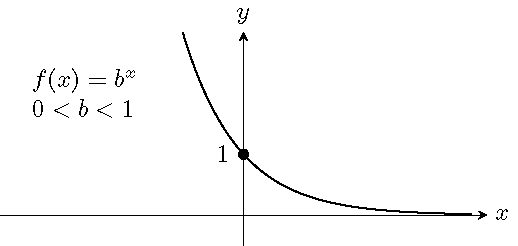
\includegraphics[scale=0.8]{figs/tikz-example-exp-function-1.png}
  
  \columnbreak

  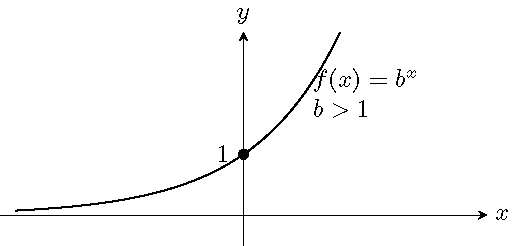
\includegraphics[scale=0.8]{figs/tikz-example-exp-function-2.png}
\end{multicols}

\begin{remark}

The exponential function \(f(x)=b^x\) is an one-to-one function: any
vertical line or any horizontal line crosses the graph at most once.
Equivalently, the equation \(b^x=c\) has at most one solution for any
real number \(c\).

\end{remark}

\subsection{The Natural Number e}

The natural number \(e\) is the number to which the quantity
\(\left(1+\dfrac1n\right)^n\) approaches as \(n\) takes on increasingly
large values. Approximately, \(e\approx 2.718281827\).

\subsection{Compound Interests}

After \(t\) years, the balance \(A\) in an account with a principal
\(P\) and annual interest rate \(r\) is given by the following formulas:

\begin{enumerate}
\item
  For \(n\) compounding periods per year:
  \(A=P\left(1+\dfrac{r}{n}\right)^{nt}\).
\item
  For compounding continuously: \(A=Pe^{rt}\).
\end{enumerate}

\begin{example}

A sum of \(\$10,000\) is invested at an annual rate of \(8\%\), Find the
balance, to the nearest hundredth dollar, in the account after \(5\)
years if the interest is compounded

\begin{enumerate}
\item
  monthly,
\item
  quarterly,
\item
  semiannually,
\item
  continuous.
\end{enumerate}

\end{example}

\begin{remark}

In the compounded investment module, the \(\frac rn\) is an
approximation of the period interest rate. Indeed, if the period rate
\(p\) satisfies the equation \((1+p)^n=1+r\), or equivalently
\(p=\sqrt[n](1+r) - 1\). Using the formula
\((1+x)^n=1+nx+\frac{n(n-1)}{2}x^2+\cdots +x^n\), one may approximately
replace \(1+r\) by \((1+\frac rn)\) and obtain the approximation
\(p\approx \frac rn\).

\end{remark}

\begin{example}

The population of a country was about 0.78 billion in the year 2015,
with an annual growth rate of about 0.4\%. The predicted population is
\(P(t)=0.78(1.004)^t\) billions after \(t\) years since 2015. To the
nearest thousandth of a billion, what will the predicted population of
the country be in 2030?

\end{example}

\subsection{Practice}

\begin{exercise}

The value of a car is depreciating according to the formula:
\(V=25000(3.2)^{-0.05x}\), where \(x\) is the age of the car in years.
Find the value of the car, to the nearest dollar, when it is five years
old.

\end{exercise}

\begin{exercise}

A sum of \$20,000 is invested at an annual rate of 5.5\%, Find the
balance, to the nearest dollar, in the account after 5 years subject to

\begin{enumerate}
\item
  monthly compounding,
\item
  continuously compounding.
\end{enumerate}

\end{exercise}

\begin{exercise}

Sketch the graph of the function and find its range.

\begin{enumerate}
\item
  \(f(x)=3^x\)
\item
  \(f(x)=\left(\frac13\right)^x\)
\end{enumerate}

\end{exercise}

\begin{exercise}

Use the given function to compare the values of \(f(-1.05)\), \(f(0)\)
and \(f(2.4)\) and determine which value is the largest and which value
is the smallest. Explain your answer.

\begin{enumerate}
\item
  \(f(x)=\left(\frac{5}{2}\right)^x\)
\item
  \(f(x)=\left(\frac23\right)^x\)
\end{enumerate}

\end{exercise}

